%% USEFUL LINKS:
%% -------------
%%
%% - UiO LaTeX guides:          https://www.mn.uio.no/ifi/tjenester/it/hjelp/latex/
%% - Mathematics:               https://en.wikibooks.org/wiki/LaTeX/Mathematics
%% - Physics:                   https://ctan.uib.no/macros/latex/contrib/physics/physics.pdf
%% - Basics of Tikz:            https://en.wikibooks.org/wiki/LaTeX/PGF/Tikz
%% - All the colors!            https://en.wikibooks.org/wiki/LaTeX/Colors
%% - How to make tables:        https://en.wikibooks.org/wiki/LaTeX/Tables
%% - Code listing styles:       https://en.wikibooks.org/wiki/LaTeX/Source_Code_Listings
%% - \includegraphics           https://en.wikibooks.org/wiki/LaTeX/Importing_Graphics
%% - Learn more about figures:  https://en.wikibooks.org/wiki/LaTeX/Floats,_Figures_and_Captions
%% - Automagic bibliography:    https://en.wikibooks.org/wiki/LaTeX/Bibliography_Management  (this one is kinda difficult the first time)
%%
%%                              (This document is of class "revtex4-1", the REVTeX Guide explains how the class works)
%%   REVTeX Guide:              http://www.physics.csbsju.edu/370/papers/Journal_Style_Manuals/auguide4-1.pdf
%%
%% COMPILING THE .pdf FILE IN THE LINUX IN THE TERMINAL
%% ----------------------------------------------------
%%
%% [terminal]$ pdflatex report_example.tex
%%
%% Run the command twice, always.
%%
%% When using references, footnotes, etc. you should run the following chain of commands:
%%
%% [terminal]$ pdflatex report_example.tex
%% [terminal]$ bibtex report_example
%% [terminal]$ pdflatex report_example.tex
%% [terminal]$ pdflatex report_example.tex
%%
%% This series of commands can of course be gathered into a single-line command:
%% [terminal]$ pdflatex report_example.tex && bibtex report_example.aux && pdflatex report_example.tex && pdflatex report_example.tex
%%
%% ----------------------------------------------------


\documentclass[english,notitlepage,reprint,nofootinbib]{revtex4-1}  % defines the basic parameters of the document
%,biblatex

% Allows special characters (including æøå)
\usepackage[utf8]{inputenc}

%\usepackage[
%backend=biber,
%style=alphabetic,
%sorting=none
%]{biblatex}
\usepackage{physics,amssymb}  % mathematical symbols (physics imports amsmath)
\include{amsmath}
\usepackage{graphicx}         % include graphics such as plots
\usepackage{xcolor}           % set colors
\usepackage{hyperref}         % automagic cross-referencing
\usepackage{listings}         % display code
\usepackage{subfigure}        % imports a lot of cool and useful figure commands
\usepackage{float}
%\usepackage[section]{placeins}
\usepackage{algorithm}
\usepackage[noend]{algpseudocode}
\usepackage{subfigure}
\usepackage{tikz}
\usepackage{xcolor}
\usetikzlibrary{quantikz}
\usepackage{pgf}
\usepackage{enumerate}


% defines the color of hyperref objects
% Blending two colors:  blue!80!black  =  80% blue and 20% black
\hypersetup{ % this is just my personal choice, feel free to change things
    colorlinks,
    linkcolor={red!50!black},
    citecolor={blue!50!black},
    urlcolor={blue!80!black}}

\usepackage{algorithm}
\usepackage[noend]{algpseudocode}
\usepackage{algpseudocode}
\bibliographystyle{apsrev4-2}



%\addbibresource{references.bib} % Imports bib file
% ===========================================
                       % self-explanatory
\begin{document}
\title{Studying classification and regression problems using neural networks}  % self-explanatory
\author{Erlend Kristensen, Mathias Mellemstuen, Magnus Selmer-Anderssen Kråkenes} % self-explanatory
\date{\today}      


\noaffiliation                            % ignore this, but keep it.

%This is how we create an abstract section.
\begin{abstract}
    In this project we looked at different methods for solving regression and classification problems and compared them with a neural network which we made. For regression we looked at gradient descent with and without a stocastich implementation, and found out that the stocastich variant performed the best. Further on we tested methods for tuning the learning rate, which proved to give better results. For classification we used logistic regression. We found out that our neural network was the best option for regression but performed poorly for classification, where logistic regression was the best. For our neural network model we also tested different activation functions to see which performed best. We tested the sigmoid, relu and leaky relu functions, and found out that sigmoid produced best results on regression, but relu was more stable and therefore probably a better option. Leaky relu was very unstable and unusable for our chosen regression data set. For classification we did not get to see much difference since our network performed poorly here.
\end{abstract}
\maketitle


% ===========================================

\section{Introduction}
\label{sec:INTRODUCTION}
% Motivate the reader, the first part of the introduction gives always a motivation and tries to give the overarching ideas
Neural networks are powerful computational systems. Their structure and function are inspired by the human brain, with nodes organized in networks processing and passing on information, mimicking neurons. This structure allows a neural network to be trained, allowing it to perform tasks without the programming of task-specific rules, making them very useful to solve complex problems. % The general idea behind artificial neural networks is to mimic the neural networks of the human brain, which is composed of billions of neurons that communicate between each other with electrical signals.  The first model of an artificial neural network was developed in 1943 by McCulloch and Pitts. 
% Få inn kilder
\\

% What we have done
In this project we will build a \textit{feed forward neural network} (FFNN) that can handle both classification problems and regression problems. We will test the ability of this network by comparing its results with results achieved using linear and \textit{logistic} regression. By analyzing the results we hope to uncover some of the pros and cons of using simple neural networks, thus giving us an indication of their usefulness and effectiveness, and also increase our understanding of which tasks they should be applied to.  
\\

% At the end of the introduction you should give a brief summary of the structure of the report
First, we will introduce the theory and methods we have utilized in section \ref{sec:METHODS}. We will then explain how we have implemented our FFNN in section \ref{sec:IMPLEMENTATION}. Our results will be presented and discussed in section \ref{sec:DISCUSSION}. We will then have an overall conclusion in section \ref{sec:CONCLUSION}, where we also suggest further work.
% Er det for mye å ha tre avsnitt i introduksjonen? Kan eventuelt slå dem sammen. 
\section{THEORY AND METHODS}
\label{sec:METHODS}

\subsection{Gradient descent}
\textit{Gradient descent} (GD) is an iterative optimization algorithm used to find local minima of a function. It works by calculating the gradient in the current position of a function, and moving in the opposite direction. That is, for a function \textit{f(x)}, 
\begin{align}
    x_{k+1} = x_{k} - \gamma \nabla f(x_{k})
\end{align}
where $\gamma$ is the \textit{learning rate}, which we will return to soon. The process is repeated for each new position, and one will therefore gradually descend towards the local minimum. We will utilize this by performing gradient descent on our cost functions, and thus find potential optimal parameter values. The number of iterations needed to find the minimum may, however, be very high, and depending on the function and the size of the data set, computing the gradient at each iteration may be computationally expensive. Methods to reduce the amount of computations have therefore been introduced.\\
One such method is \textit{momentum gradient descent}. In momentum gradient descent we extend the standard GD method by introducing memory about the previous step and a new hyperparameter \textit{momentum} . The next position in the iteration is therefore influenced by the previous change weighted by the momentum.
\begin{align}
    x_{k+1} = x_{k} - (\gamma \nabla f(x_{k}) + momentum * \Delta x)
\end{align}
This can reduce the effect of sudden fluctuations or noise in the function, while also boosting the speed of the descent in directions with persistent gradients [Hjorth-Jensen (\ref{ref:Morten}), sec. 7.8], thus increasing the speed of the optimization process.
\\
Another method of making the GD method less computationally expensive is to approximate the gradient using only a subset of the data. % Formel?
By dividing the data set into smaller batches, called \textit{mini-batches}, and calculating the gradient using randomly chosen mini-batches, the number of calculations is reduced, while also introducing randomness, thus reducing the probability of our optimization process getting stuck in local minima or saddle points. % Gjelder dette og for saddle points eller kun lokale minima?
This is the basis for \textit{stochastic gradient descent} (SGD) with mini-batches. The SGD step algorithm is 
\begin{align}
    x_{k+1} = x_{k} - \gamma_{k} \sum_{i \in B_{j}}^{m} \nabla_{x} c_{i}(B_{i}, x)
\end{align}
where m is the number of mini-batches, i is a random number between 1 and m, and $B_{i}$ is mini-batch number i. We call an iteration over the training set, that is, the number of mini-batches, an \textit{epoch}. The amount of epochs we have is a hyperparameter, and we will test different amounts of epochs to find a number which provides a good performance, while also being time efficient. 


\subsection{Learning rate}
While the direction of the descent is determined by the gradient, the speed of the descent, how fast the GD methods converge towards the minima, is determined by the learning rate, $\gamma$, which is a value between 0 and 1. More specifically, the learning rate determines the step size at each iteration. A large learning rate should therefore produce a faster descent, as the number of iterations can be reduced. However, a gradient is only true in its exact position, and using the same gradient over a large step size could therefore provide unpredictable and inaccurate feedback, and there is a chance that certain minima are missed.
On the other hand, using a very small step size can greatly increase the number of necessary iterations, thus increasing computation time. We therefore want to use a learning rate which balances accuracy and number of necessary iterations. % Mulig å omformulere? Ikke helt fornøyd med setningen
\\
\\
The most simplistic way to find a learning rate is to use a single learning rate size throughout the entire gradient descent process. This size can be chosen arbitrarily, or it can be found by testing different sizes and picking the preferred value. However, as the GD method is sensitive to the choice of learning rate, this method can provide poor results. We can improve results by utilizing a \textit{learning rate schedule}. Learning rate schedules are algorithms which continuously update an initial learning rate during training. There are several different learning rate schedules. % Si noe mer her?
We will primarily utilize a time based schedule by introducing a time decay rate, reducing our learning rate at each iteration:
\begin{align}
    \gamma_{k} = \frac{t_{0}}{t + t_{1}},
\end{align}
where $t_{0}$ and $t_{1}$ are constants where $t_{0} < t_{1}$, and t, representing time, is determined by the current amount of iterations we have completed. % Skriv om?
Utilizing this time decay rate we prevent our gradient descent process from jumping back and forth over a minimum.
\\

While learning rate schedules may provide improved results, the learning rates  are still % dependent on manually chosen hyperparameters, and they are 
limited to the direction of the steepest descent. We will therefore test % implement?
three different adaptive gradient descent methods, \textit{AdaGrad}, \textit{Root Mean Squared Propagation} (RMSprop), and \textit{Adam}, which are designed to allow us to take larger steps in shallow directions and smaller steps in steep directions [Hjorth-Jensen (\ref{ref:Morten}), sec. 7.8]. % Er det riktig å bruke kilde på dette?
\\

AdaGrad is an algorithm which adapts the learning rates of the parameters depending on the size of their partial derivatives. The learning rates decrease more for parameters with large partial derivatives than for parameters with small partial derivatives [Goodfellow et al (\ref{ref:Goodfellow et al}), p.303]. In other words, the step size is smaller in steep directions than in more shallow directions. The update rule for AdaGrad is:
% https://www.deeplearningbook.org/contents/optimization.html, side 303
\begin{align} \label{formula 4}
    x_{k+1} = x_{k} - \frac{\gamma_{0}}{\delta I + \sqrt{G_{k}}}\odot g_{k},
\end{align}
where I is the identity matrix, $g_{k}$ is the gradient in the current position ($x_{k}$), and $G_{k}$ is the outer product of all previous gradients, that is
\begin{align} 
    G_{k} = \sum_{i=1}^{k} g_{i}g_{i}^{T}.
\end{align}
We add a very small number, $\epsilon$, to $G_{k}$ to prevent division by 0, and to make the algorithm less computationally expensive, we use only the diagonal elements of $G_{k}$.
% AdaGrad functions very well with convex functions, but less good with non-convex functions
\\

The RMSprop algorithm is a slight modification of AdaGrad. The update algorithm with RMSprop is actually the same as with AdaGrad (\ref{formula 4}), but with a different way of calculating $G_{k}$:
\begin{align} \label{formula 6}
    G_{k} = \rho G_{k-1} + (1 - \rho) \sum_{i=1}^{k} g_{i}g_{i}^{T}
\end{align}
where $\rho$ is the decay rate, which is a new hyperparameter. $G_{k}$ now represents the \textit{exponentially weighted moving average} (EWMA) of the second moment of the gradient, with $\rho$ as weight. % Ha med denne (forrige) setningen?
The calculation of $G_{k}$ shows that RMSprop introduces a memory about the previous iteration, mimicking the function of momentum. The RMSprop algorithm is designed to improve performance in non-convex settings compared to AdaGrad [Goodfellow et al (\ref{ref:Goodfellow et al}), p.303]. \\
% Skal vi ha med sidetall i kilder?

Adam builds further on RMSprop by adding another decay rate hyperparameter, and by performing a bias correction. We have $m_{k}$, the EWMA of the first moment, given by
\begin{align}
    m_{k} = \rho_{1} m_{k-1} + (1 - \rho_{1}) g_{k}, 
\end{align}
and $G_{k}$, the EWMA of the second moment, calculated as in formula (\ref{formula 6}), except with $\rho_{2}$ instead of $\rho$. We then correct for the biases with
\begin{align}
    \hat{m}_{k} = \frac{m_{k}}{1-\rho_{1}^{k}}
\end{align}
and
\begin{align}
    \hat{G}_{k} = \frac{G_{k}}{1-\rho_{2}^{k}}.
\end{align}
The introduction of bias correction makes adam relatively robust when it comes to choice of hyperparameter values [Goodfellow et al (\ref{ref:Goodfellow et al}), p.306]. We use these bias corrected values when we calculate the update, which is given by
\begin{align}
    x_{k+1} = x_{k} - \gamma_{k} \frac{\hat{m}_{k}}{\sqrt{\hat{G}_{k}} + \epsilon}
\end{align}
\\

We will test both GD and SGD with and without these methods for altering the learning rate, and compare their results. For simplicity, our FFNN will only implement one of these methods. % Er dette riktig? Og i så fall, er dette riktig sted å skrive det?

\subsection{Classification}
Linear regression uses input in order to predict the value of a continuous variable. Often, however, we are interested in determining whether or not something belongs in specific categories. In these cases, we are not interested in some continuous variable, but rather discrete variables, representing different classes. There are several different methods to solve classification problems, one of which is logistic regression, a so-called "soft classifier". It is called a soft classifier as it utilizes an otherwise continuous function, in our case the \textit{Sigmoid function}, and gives an output, a discrete value, based on whether or not the result of the Sigmoid function is above a predetermined threshold. The Sigmoid function represents the probability that, given the input, the output belongs in a specific class. \\
%  The prediction is done by multiplying our input values with our weights, and running the results through the sigmoid function. Then, to predict each class, it goes through the list of values and assigns each value that is over a set threshold (usually set at 0.5 which means its $50 \%$ or more accurate to be true), and if it is under the threshold value, it is assigned to class 0. 

%¤ Cross entropy? \\ % Bruker vi dette? Nei
We will use logistic regression as a comparison to test our FFNN's ability to classify data. However, in classification problems, where we are interested in the class determined by the output, rather than the output value itself, performance measures such as \textit{mean squared error} (MSE) and \textit{$R^2$} are less useful. We therefore use other measures of performance, such as the \textit{accuracy} measure and the \textit{confusion matrix}. 
\\
The accuracy of a model is simply the ratio of correct predictions. That is
\begin{align}
    accuracy = Correct Predictions / Total Predictions
\end{align}
An accuracy of 1 means that the model has correctly predicted all cases. The accuracy score is, however, sensitive to imbalanced data, as a faulty model can give a high accuracy if it only predicts the most common class. Another method of assessing model performance is to create a confusion matrix. The confusion matrix is a matrix containing the number of correct and incorrect predictions for each class, providing a clear overview of the model performance, while also providing an indication of whether or not the input data is imbalanced. 

%For classification we will test our FFNN against a regression method called logistic regression. Logistic regression is primarily used for classification problems due to the fact that it uses the sigmoid function (which we will mention more on later) to do its predictions. The prediction is done by multiplying our input values with our weights, and running the results through the sigmoid function. Then to predict each class, it goes through the list of values and assigns each value that is over a set threshold (usually set at 0.5 which means its $50 \%$ or more accurate to be true), and if it is under the threshold value, it is assigned to class 0. 
% Jeg har prøvd å implementere dette i teksten over
\\



\section{Implementation}\label{sec:IMPLEMENTATION}

\subsection{Cost functions}
When implementing GD, we have to use a so called \textit{Cost function} to approximate the gradients. We will use two methods to implement the gradient descent algorithm. The first one is \textit{Ordinary least squared} (OLS), which calculates the gradient using the cost function
\begin{align*}
    \frac{1}{n}*\sum ((y-x).\beta)^2)
\end{align*}
where $\beta$ is the weights we train our network for, $x$ is the input values and $y$ is the values we want to approximate. 
\\
\\
The other method we want to implement is Ridge regression, which calculates the graidients as by adding an l2-regularization
\begin{align*}
    \lambda \sum \beta^2
\end{align*}
where $\lambda$ is a constant which is greater or equal to $0$. This will help with penalizing the sum of squares of the parameter (weights), which is called \textit{weight decay}. The larger $\lamda$ is, the more we shrink the weights [T.hastie, \ref{ref:HASTIE}].
\\
\\
As stated earlier, we will use MSE to test the accuracy of our models when the problem is regression, which can be implemented as
\begin{align*}
    \frac{1}{n}\sum (y - y_{pred})^2
\end{align*}

\subsection{Feed Forward Neural Network}
As stated in our introduction, the point of an artificial neural network was to mimic the human brain. The method of doing this is to make a large network with multiple ''neurons'', which in this case will be what we will call a \textit{hidden node}. The network works by taking in a certain amount of information as what we call \textit{input nodes}, and running them through the networks multiple \textit{hidden layers}, which consists of a set amount of hidden nodes. For each layer we run the output through an \textit{activation function}, until we eventually end up with the output layer, which will give us the prediction from the network.
%\begin{figure}[H]
%    \centering
%    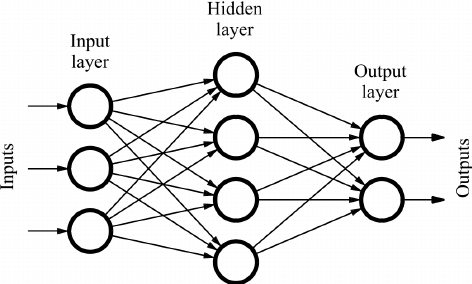
\includegraphics[width=0.45\textwidth]{FYS-STK/Prosjekt_2/FFNN_illustration.png}
%    \caption{Visual representation of a neural network.}
%    \label{fig:1}
%\end{figure}
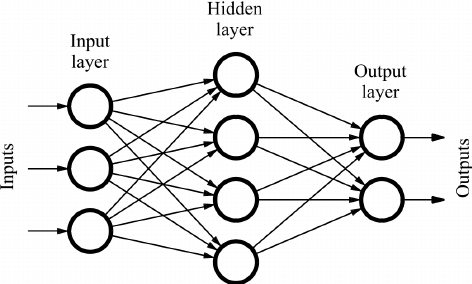
\includegraphics[width=0.45\textwidth]{FYS-STK/Prosjekt_2/FFNN_illustration.png}
\caption{Figure 1: Visual representation of a neural network.}

This is the first step for the neural network, and is what we call the \textit{feed forward} method, which can be written with these equations:

\begin{align*}
    z_1 &= x*w_1 + b_1 \\
    a_1 &= f(z_1) \\
    \\
    z_i &= a_{i-1}*w_i + b_i \\
    a_i &= f(z_i) \\
    \\
    z_n &= a_{n-1}*w_n + b_n \\
    a_n &= z_n
\end{align*}
where $i = 2,...,n$ and $n$ represents the number of hidden layers, $w$ is our networks weights, $x$ is the input values and $b_i$ is the associated bias. For regression problems, our predicted result will be $z_n$, but for classification problems, we will get the predicted result as $\frac{e^z}{\sum e^z}$.
\\
Now that we have a prediction, we want to test how good this prediction is, and tune our model so that our next prediction will be better. This step is what we call \textit{backpropagation}. The algorithm for backpropagation is as follows:

\begin{align*}
    error_1 &= y_{pred} - y_{true} \\ 
    error_i &= error_{i-1} * w_{n-i} * f'(z_{n-i-1}) \\ 
    \Delta w_i &= a_{n-1-i} * error_i \\ 
    \Delta b_i &= \sum error_i \\ 
    \Delta w_n &= x * error_n \\ 
    \Delta b_n &= \sum error_n \\ 
    w_i &= w_i - \gamma \Delta w_{n-i} \\ 
    b_i &= b_i - \gamma \Delta b_{n-i}
\end{align*}
where $y_{pred}$ is our predicted outcome, $y_{true}$ is the correct result, $f'$ is the derivative of our activation function.
The reason the algorithm might seem weird, such as we update a weight $w_i$ with $\Delta w_{n-i}$, is because we go backwards in backpropagation, so the last derivative we calculate will correspond to the first weight (the input weight). 
\\
Now that we have explained the basis of how we will build our neural network, we want to look at the activation functions which we mentioned above. The reason for implementing an activation function is to introduce non-linearity in our neural network, which allows our network to develop complex representations that would not be possible with a simple linear regression.
The different activation functions we will look at are

\begin{align*}
\textit{sigmoid} &= \frac{1}{1 + e^{-z}} \\
\textit{relu} &= max(0,z) \\ 
\textit{leaky relu} &= max(0.01*z, z)
\end{align*}

and their derivatives are

\begin{align*}
\Delta \textit{sigmoid} &= f(z) * (1-f(z)) \\
\Delta \textit{relu} &= \textit{1 if z $>$ 0, otherwise 0} \\ 
\Delta \textit{leaky relu} &= \textit{1 if z $>$ 0, otherwise 0.01}
\end{align*}

The sigmoid function will normalize the output to a range between $0$ and $1$, giving a probability of the input value, which will make it better suited for classification problems. However, it is highly expensive computation wise, and it also suffers poor learning when a neuron is either its maximum value or minimum value, which means that $f(z) = \textit{0 or 1}$, such that the gradient is $0$. This means there is no update in the weights, and the network will not learn anything from these neurons. This is called saturated neurons.
\\
Relu and leaky relu however are fast to compute, and since its derivative is always positive for positive inputs, it means that we will never have a saturated neuron for any positive input values, and for leaky relu, we will never have a saturated neuron, even for negative values [S.Dorsaf (\ref{ref:DORSAF})].
\\
\\
We will study these activation functions more and compare their results to see which perform best for problems such as regression and classification.


\subsection{Data sets}
The data we will use as our classification problem is the \textit{breast cancer Wisconsin data set} downloaded from the sklearn library. % Link?
This is a well known data set which is typically used in machine learning exercises. % Er dette riktig? Gjerne omformuler
It contains 569 samples with data about several different attributes of tumor cases, including whether the tumor is benign (357 cases) or malignant (212 cases). 
\\
\\
The data we use for testing our regression problems is the \textit{Franke function}, which is a $2$-dimensional function (see Appendix \ref{eq:FrankeFunction}), and is often used to train networks for regression problems due to its complexity. 
%\begin{figure}[H]
%    \centering
%    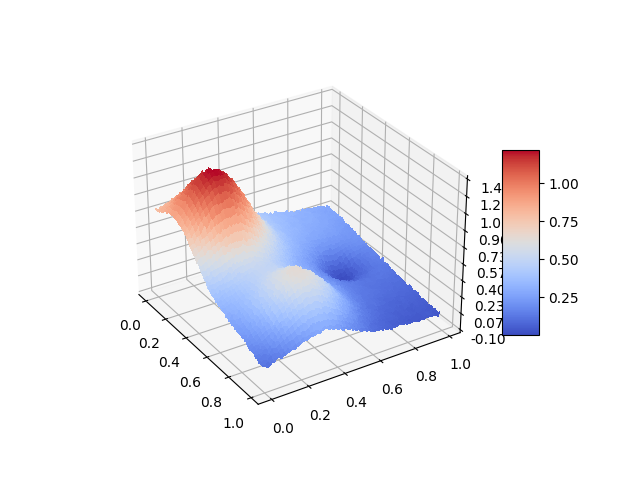
\includegraphics[width=0.45\textwidth]{FYS-STK/Prosjekt_2/Franke.png}
%    \caption{Visual representation of the Franke function using $x,y \in [0,1]$.}
%    \label{fig:2}
%\end{figure}
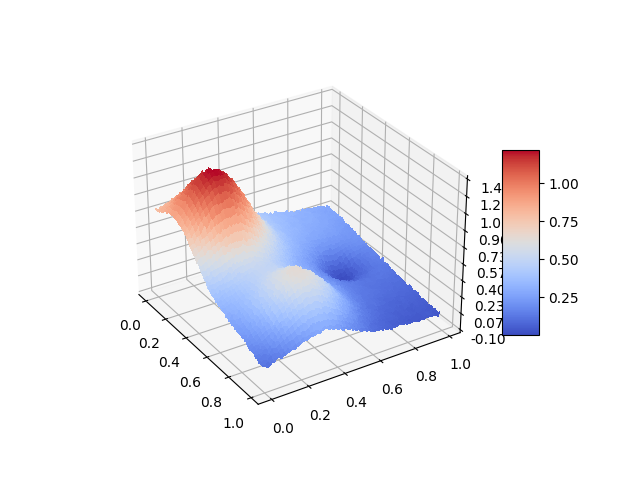
\includegraphics[width=0.45\textwidth]{FYS-STK/Prosjekt_2/Franke.png}
\caption{Figure 2: Visual representation of the Franke function using $x,y \in [0,1]$.}

\section{RESULTS AND DISCUSSION}\label{sec:DISCUSSION}
As stated earlier, we want to look at both GD and SGD, with and without a tuning of the learning rate. 
%\begin{figure}[H]
%    \centering
%    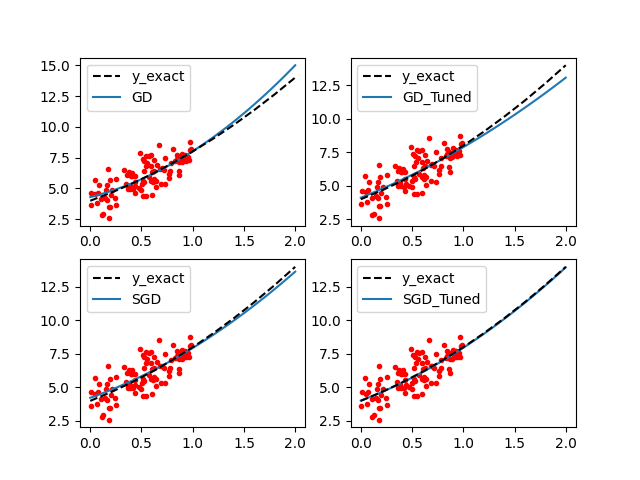
\includegraphics[width=0.45\textwidth]{FYS-STK/Prosjekt_2/A4_OneTuned.png}
%    \caption{Plot of GD and SGD with and without tuning the learning rate, approximating the function $f(x) = x^2 + 3x + 4$.}
%    \label{fig:3}
%\end{figure}
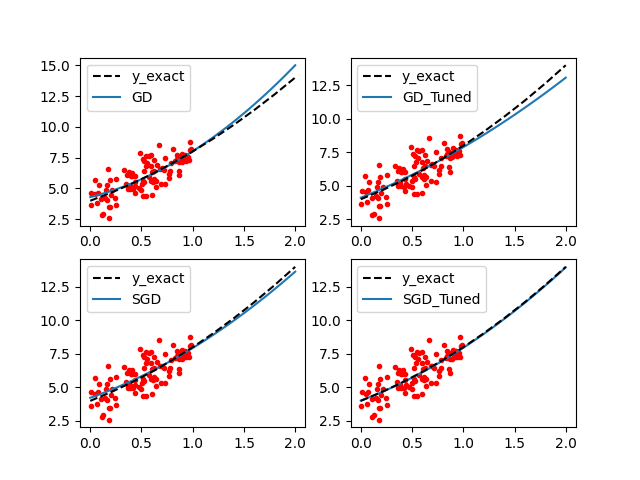
\includegraphics[width=0.45\textwidth]{FYS-STK/Prosjekt_2/A4_OneTuned.png}
\caption{Figure 3: Plot of GD and SGD with and without tuning the learning rate, approximating the function $f(x) = x^2 + 3x + 4$.}
\\
\\
Here we used a set learning rate of $0.1$ with 200 iterations, with a momentum of 0.1 and a batch size of 5 for the stocastich variants. These parameters were found when testing our models, and seemed to be the best options. We clearly observe that both SGD with and without tuning perform better than a standard GD, even with tuning. It is also clear that the SGD with learning rate tuning performs better than without, giving us a result that is near perfectly aligned with the actual result. It is therefore safe to say that tuning the learning rate as we run through the iterations is a good way to optimize our solution. The only problem we could run into with such a good approximation, is over-fitting, which means that our trained model works well on a certain problem, but not well in general. We also tested the OLS implementation vs the Ridge implementation for SGD with a tuned learning rate, and got a MSE of $0.0271$ for OLS and $0.6629$ for Ridge. This seems to indicate that Ridge is far worse than OLS, but this could also be due to the function we have chosen to use, and we will therefore look more into this later on.
\\
\\
We now want to compare these models with our neural network. We first look at how our network approximates the same function as used for GD and SGD.
%\begin{figure}[H]
%    \centering
%    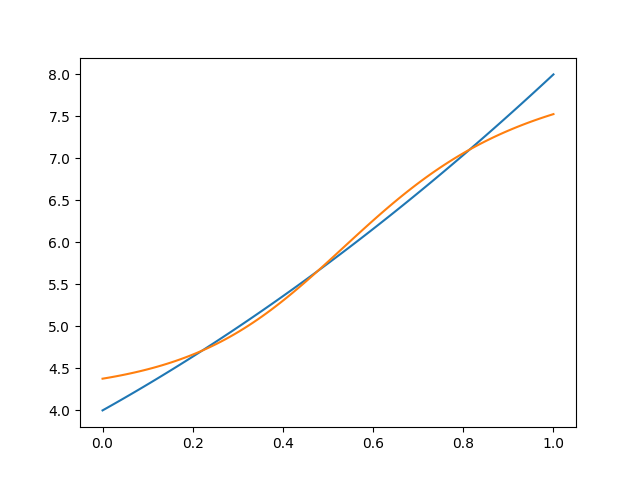
\includegraphics[width=0.45\textwidth]{FYS-STK/Prosjekt_2/FFNN prediction.png}
%    \caption{Plot our neural network approximating the function $f(x) = x^2 + 3x + 4$}
%    \label{fig:4}
%\end{figure}
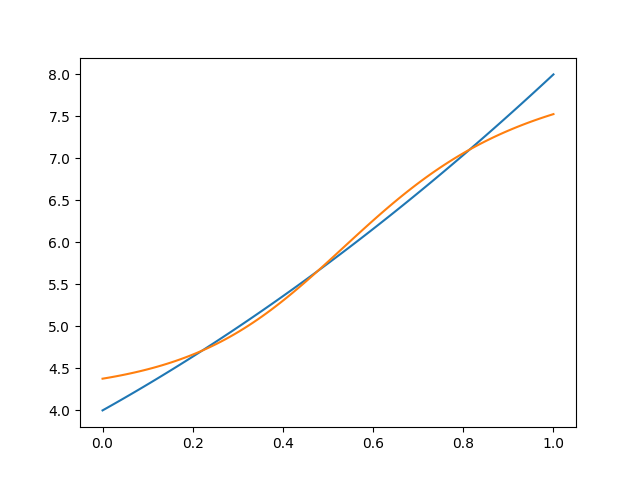
\includegraphics[width=0.45\textwidth]{FYS-STK/Prosjekt_2/FFNN prediction.png}
\caption{Figure 4: Plot of our neural network approximating the function $f(x) = x^2 + 3x + 4$}
\\
Here we used the same hyperparameters as we used for gradient descent, with layer sizes $3,5,3$. We see a more complex output here, not as linear as the predictions made from gradient descent. This is to be expected since we used the sigmoid activation function, which will turn the problem from a linear problem to a complex one. Even though our nerual network in this example seems to be outperformed by the multiple gradient descent variants, we can again think of over-fitting. With our neural network here, it makes a general assumption of the problem, which could in most cases be a a better model.
\\
To further study this we will look at a more complex function, the Franke function. Here we will test our models with a variety of values for the hyperparameters. The first we will look at are our SGD models for Ridge and OLS. We will run tests for multiple hyper parameters to get a better understanding of which parameters and models are the best. We will simulate the franke function using $x,y \in [0,1]$ with $100 \times 100$ data points each.
%\begin{figure}[H]
%    \centering
%    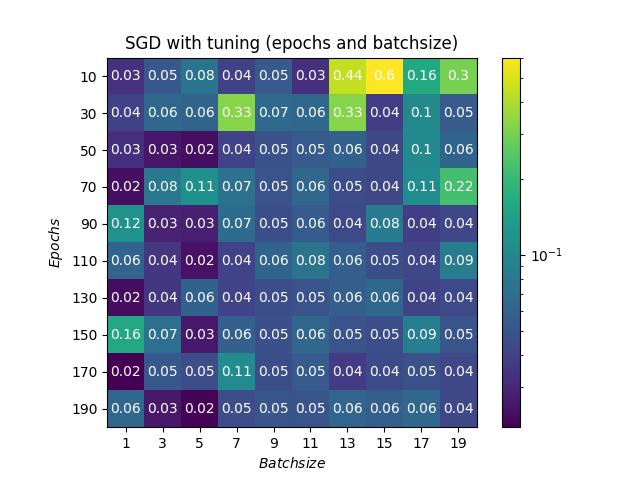
\includegraphics[width=0.45\textwidth]{FYS-STK/Prosjekt_2/SGD with tuning (epochs and batchsize).png}
%    \caption{Heatmap of our SGD model (with OLS) tested for multiple batchsizes and iterations (epochs) using the Franke function.}
%    \label{fig:5}
%\end{figure}
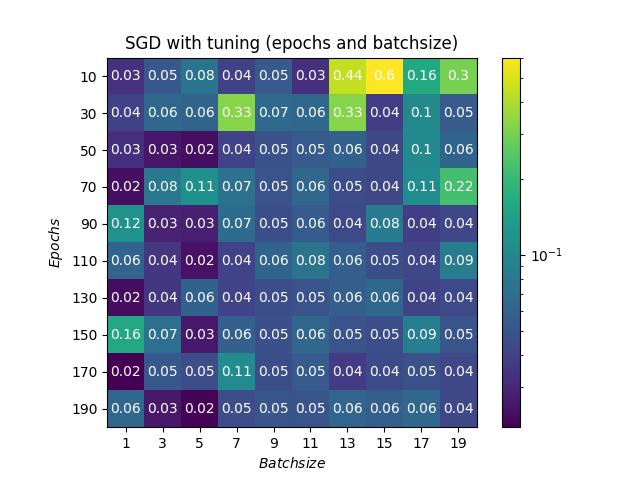
\includegraphics[width=0.45\textwidth]{FYS-STK/Prosjekt_2/SGD with tuning (epochs and batchsize).png}
\caption{Figure 5: Heatmap of our SGD model (with OLS) tested for multiple batchsizes and iterations (epochs) using the Franke function.}
We see here that the optimal values seem to be about 110 iterations and a batchsize of 5.

%\begin{figure}[H]
%    \centering
%    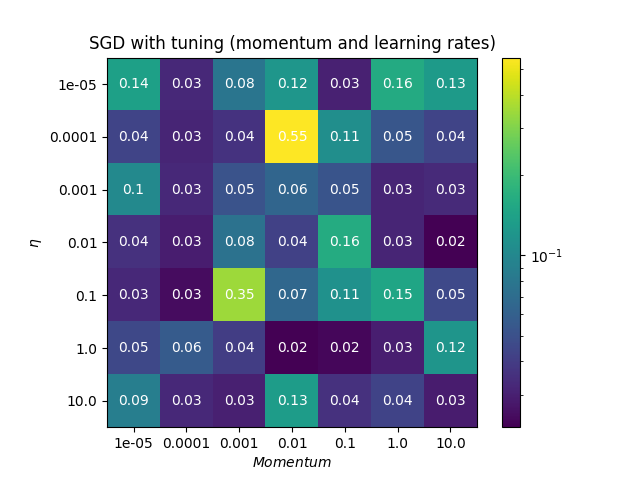
\includegraphics[width=0.45\textwidth]{FYS-STK/Prosjekt_2/SGD with tuning (momentum and learning rates).png}
%    \caption{Heatmap of our SGD model (with OLS) tested for multiple momentum and learning rate values using the Franke function.}
%    \label{fig:6}
%\end{figure}
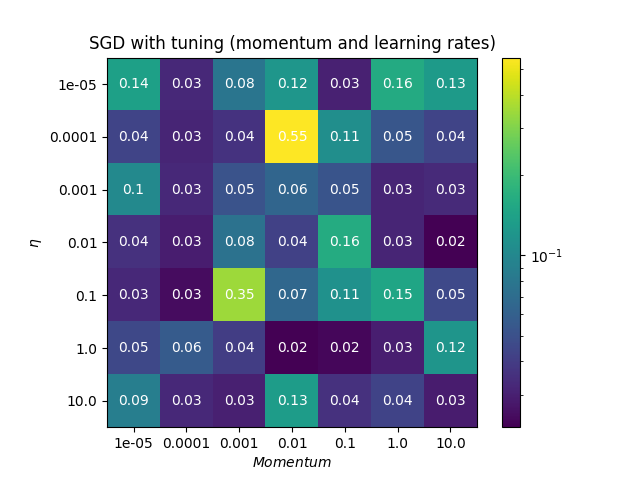
\includegraphics[width=0.45\textwidth]{FYS-STK/Prosjekt_2/SGD with tuning (momentum and learning rates).png}
\caption{Figure 6: Heatmap of our SGD model (with OLS) tested for multiple momentum and learning rate values using the Franke function.} \\
\\
We see here that the optimal values seem to be a momentum of 0.01 and a learning rate of 1, however this could be good for this specific problem, and usually a high learning rate will not perform well for every problem, so setting the learning rate to 0.01 could be a good choice.

%\begin{figure}[H]
%    \centering
%    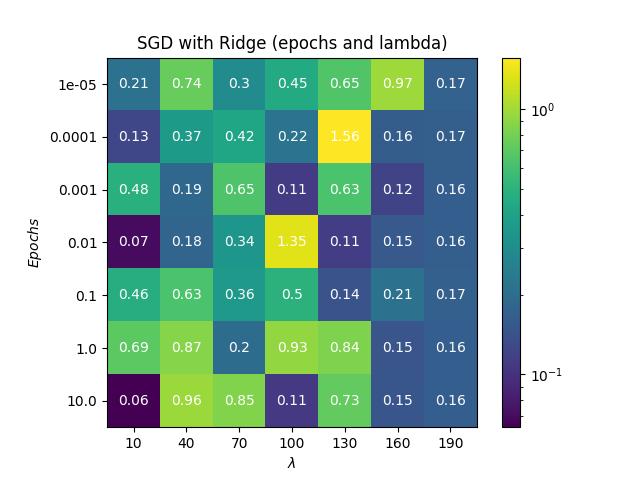
\includegraphics[width=0.45\textwidth]{FYS-STK/Prosjekt_2/SGD with Ridge (epochs and lambda).png}
%    \caption{Heatmap of our SGD model (with Ridge regression) for multiple values of $\lambda$ and iterations. Here we used the optimal values found from OLS to see the difference between the two.}
%    \label{fig:7}
%\end{figure}
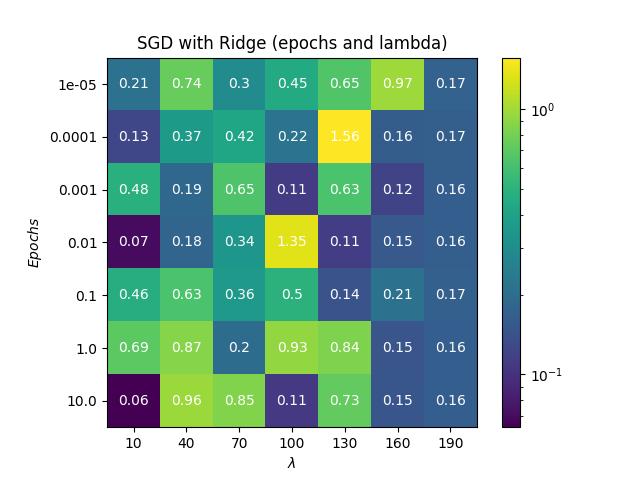
\includegraphics[width=0.45\textwidth]{FYS-STK/Prosjekt_2/SGD with Ridge (epochs and lambda).png}
\caption{Figure 7: Heatmap of our SGD model (with Ridge regression) for multiple values of $\lambda$ and iterations. Here we used the optimal values found from OLS to see the difference between the two.}

%\begin{figure}[H]
%    \centering
%    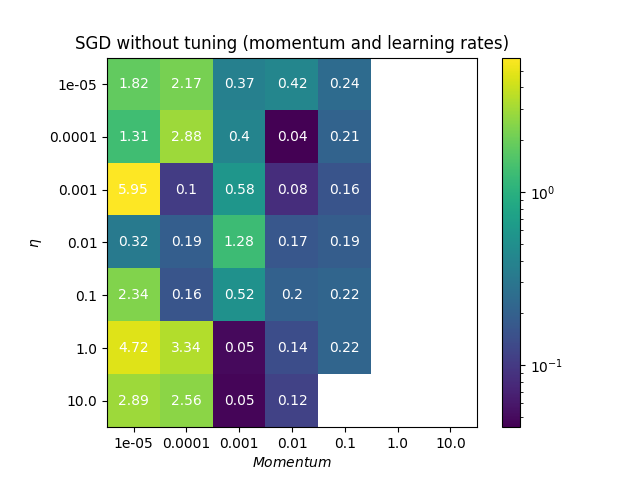
\includegraphics[width=0.45\textwidth]{FYS-STK/Prosjekt_2/SGD without tuning (momentum and learning rates).png}
%    \caption{Heatmap of our SGD model (with OLS, without tuning) tested for multiple momentum and learning rate values using the Franke function.}
%    \label{fig:8}
%\end{figure}
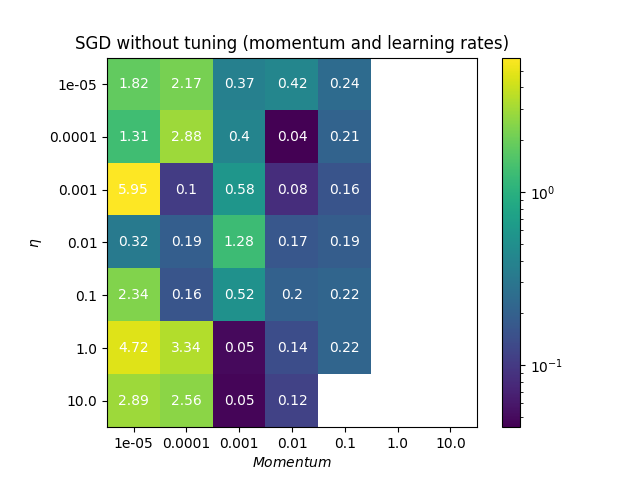
\includegraphics[width=0.45\textwidth]{FYS-STK/Prosjekt_2/SGD without tuning (momentum and learning rates).png}
\caption{Figure 8: Heatmap of our SGD model (with OLS, without tuning) tested for multiple momentum and learning rate values using the Franke function.}
\\
\\
As we see on these heatmap plots, it seems that OLS definitely outperforms Ridge using the Franke function just as we saw with our second order equation. However, Ridge is faster computation wise, and as we see some of the better results on ridge are very close to being as good as the best results for OLS. So we with different parameters and different training data, ridge might outperform, but for our chosen data is seems that OLS is the better option. 
\\
We also clearly see with our last heatmap, which is a headmap of SGD without tuning, just how important tuning our learning rate is. Here, the white space represents values where the MSE got above 2000 or higher, which shows us how quickly SGD without tuning will converge with poorly chosen parameters.
\\
\\
We will now do the same simulation using our neural network. We start by using the sigmoid function and get the following result.
%\begin{figure}[H]
%    \centering
%    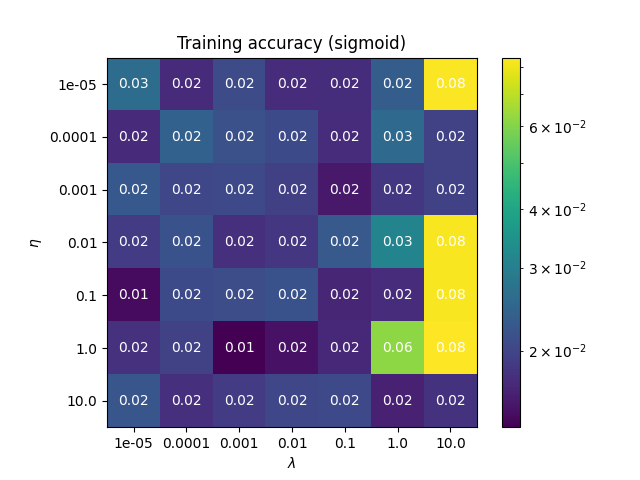
\includegraphics[width=0.45\textwidth]{FYS-STK/Prosjekt_2/Training accuracy (sigmoid).png}
%    \caption{Heatmap of our neural network (using sigmoid) tested for multiple momentum and learning rate values using the Franke function. We used a set number of $100$ iterations and a batch size of $5$ to best compare with SGD.}
%    \label{fig:9}
%\end{figure}
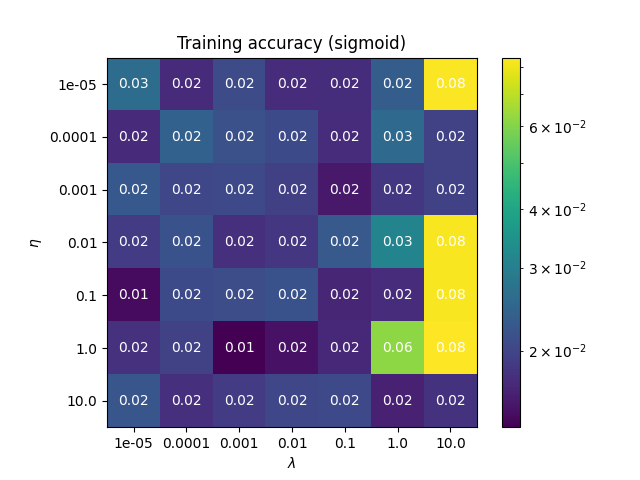
\includegraphics[width=0.45\textwidth]{FYS-STK/Prosjekt_2/Training accuracy (sigmoid).png}
\caption{Figure 9: Heatmap of our neural network (using sigmoid) tested for multiple momentum and learning rate values using the Franke function. We used a set number of $100$ iterations and a batch size of $5$ to best compare with SGD.}
\\
\\
As we can see, our network seems to outperform SGD quite well. Its optimal solutions are a bit better, and it doesn't have nearly as high of a variance in its values as SGD did, with all of our neural networks MSE values being under $0.1$, while SGD had one as high as $0.55$, even with learning rate tuning.
\\
It seems to be safe to conclude that our neural network works better than all the other regression methods, both in optimality and stability. This can also be seen when studying the output after a set amount of epochs as seen bellow.
%\begin{figure}[H]
%    \centering
%    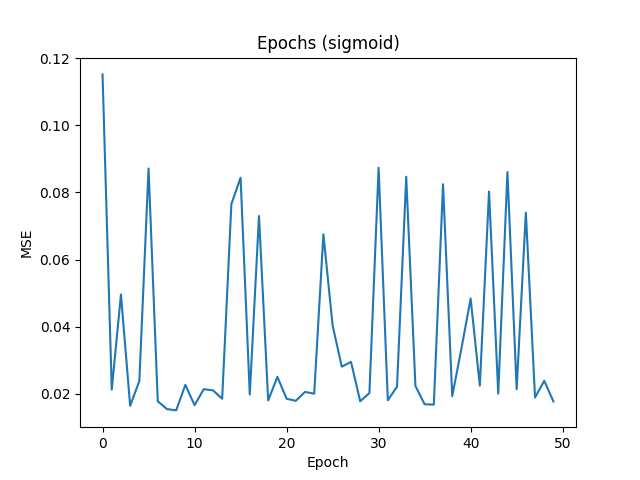
\includegraphics[width=0.45\textwidth]{FYS-STK/Prosjekt_2/Epochs (sigmoid).png}
%    \caption{Plot of change in MSE when varying amount of epochs for our neural network using the sigmoid function.}
%    \label{fig:10}
%\end{figure}
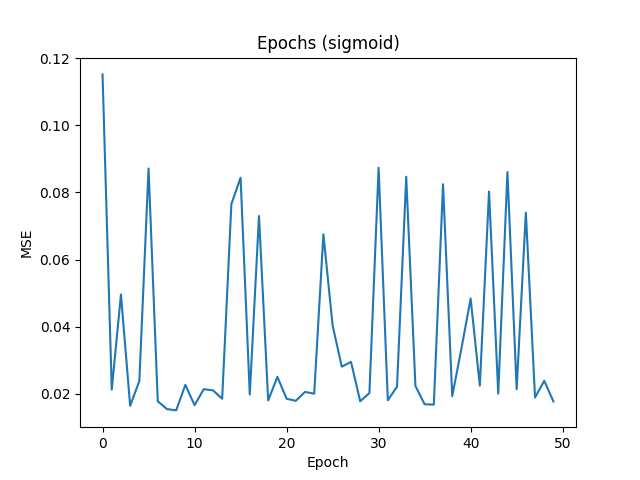
\includegraphics[width=0.45\textwidth]{FYS-STK/Prosjekt_2/Epochs (sigmoid).png}
\caption{Figure 10: Plot of change in MSE when varying amount of epochs for our neural network using the sigmoid function.}
\\
\\
Here we used a batch size of $5$ as usual to best compare. We clearly see after only few epochs that the neural network closes inn on an optimal value. It is also important to note that since we also use a stocastich method on our neural network, we will have two loops that we run through. The amount of epochs refers to the outmost loop, while the inner loop has a set amount depending on the size of the data set. This amount is calculated in the same way for our SGD implementation aswell as our neural network. Therefore we can clearly observe that our network learns fast, but we see a solid amount of fluctuation in our MSE values, not too different from what the heatmap of our SGD implementation showed. Therefore we can not conclude that our model is as stable as our heatmap might have made us believe. 
\\
\\
We will now investigate how the different uses of activation functions impact the results from our neural network. As stated previously, we will use relu and leaky relu. We do the same simulations for these two as we did with sigmoid.
%\begin{figure}[H]
%    \centering
%    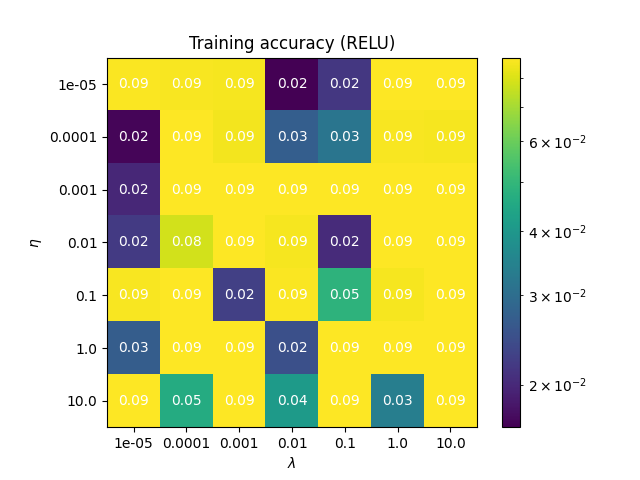
\includegraphics[width=0.45\textwidth]{FYS-STK/Prosjekt_2/Training accuracy (RELU).png}
%    \caption{Heatmap of our neural network (using relu) tested for multiple momentum and learning rate values using the Franke function. We used same number of epochs and same batch size as with sigmoid}
%    \label{fig:11}
%\end{figure}
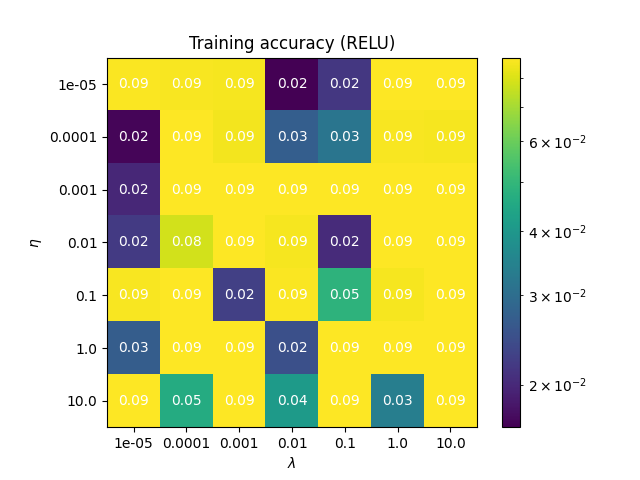
\includegraphics[width=0.45\textwidth]{FYS-STK/Prosjekt_2/Training accuracy (RELU).png}
\caption{Figure 11: Heatmap of our neural network (using relu) tested for multiple momentum and learning rate values using the Franke function. We used same number of epochs and same batch size as with sigmoid}

%\begin{figure}[H]
%    \centering
%    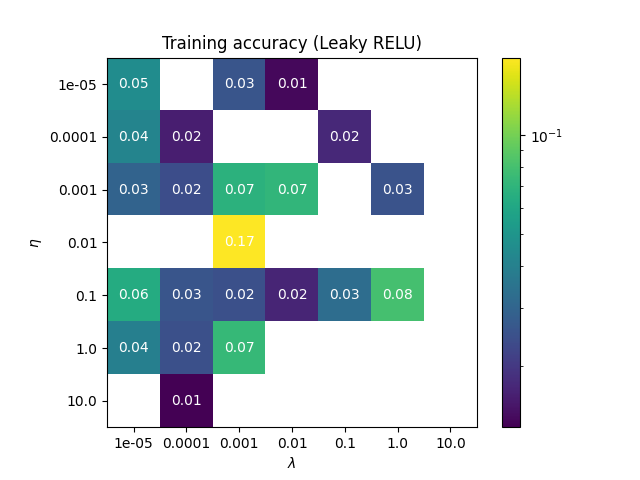
\includegraphics[width=0.45\textwidth]{FYS-STK/Prosjekt_2/Training accuracy (Leaky RELU).png}
%    \caption{Heatmap of our neural network (using leaky relu) tested for multiple momentum and learning rate values using the Franke function. We used same number of epochs and same batch size as with sigmoid}
%    \label{fig:12}
%\end{figure}
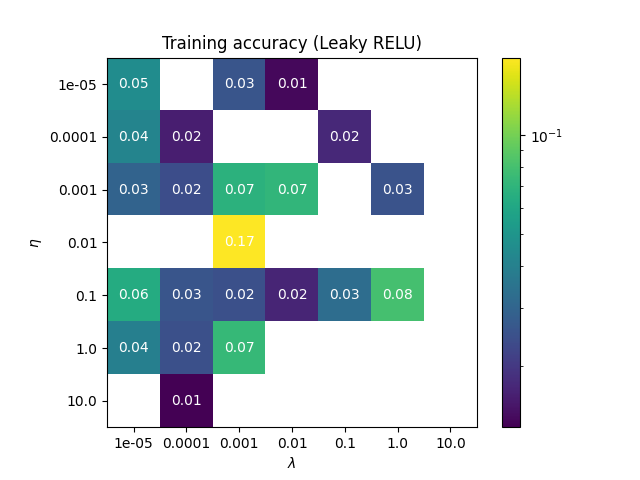
\includegraphics[width=0.45\textwidth]{FYS-STK/Prosjekt_2/Training accuracy (Leaky RELU).png}
\caption{Figure 12: Heatmap of our neural network (using leaky relu) tested for multiple momentum and learning rate values using the Franke function. We used same number of epochs and same batch size as with sigmoid}
\\
\\
As we see on these heatmaps, relu and leaky relu definitely seem more unstable than sigmoid was, with the white spaces on the leaky relu plot representing MSE values converging. Just looking at these plots, it seems that sigmoid is clearly a better option. However, we will further investigate this by plotting the MSE for a different amount of epochs as we did with sigmoid. 

%\begin{figure}[H]
%    \centering
%    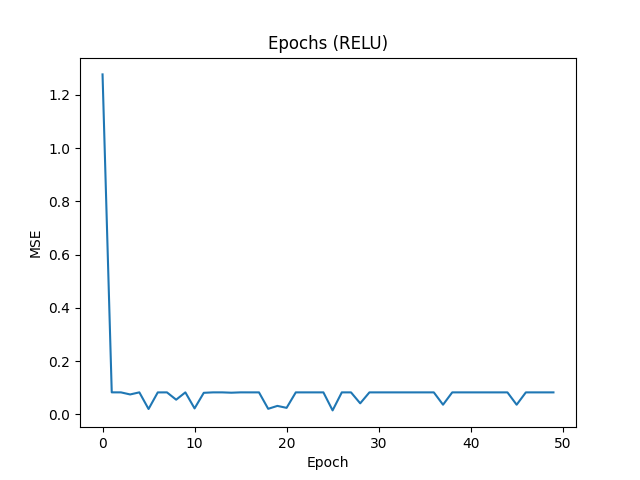
\includegraphics[width=0.45\textwidth]{FYS-STK/Prosjekt_2/Epochs (RELU).png}
%    \caption{Plot of change in MSE when varying amount of epochs for our neural network using the relu function.}
%    \label{fig:13}
%\end{figure}
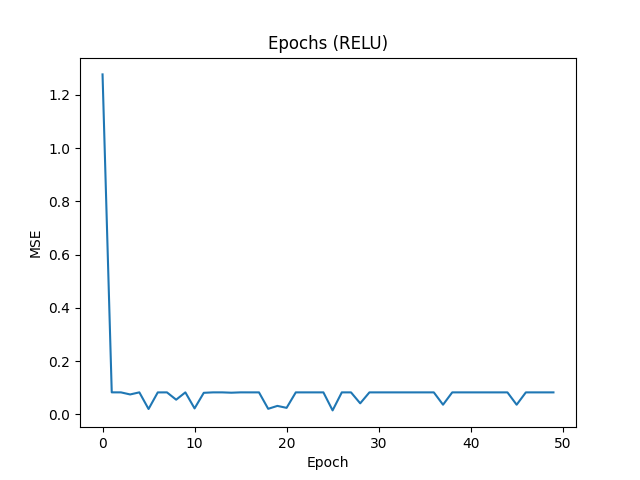
\includegraphics[width=0.45\textwidth]{FYS-STK/Prosjekt_2/Epochs (RELU).png}
\caption{Figure 13: Plot of change in MSE when varying amount of epochs for our neural network using the relu function.}

%\begin{figure}[H]
%    \centering
%    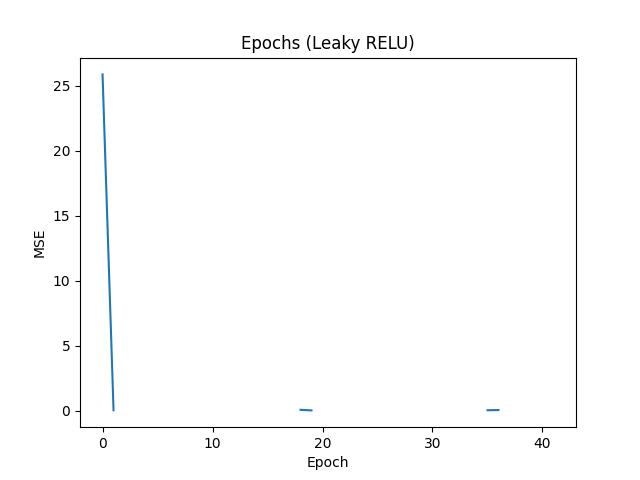
\includegraphics[width=0.45\textwidth]{FYS-STK/Prosjekt_2/Epochs (Leaky RELU).png}
%    \caption{Plot of change in MSE when varying amount of epochs for our neural network using the leaky relu function.}
%    \label{fig:14}
%\end{figure}
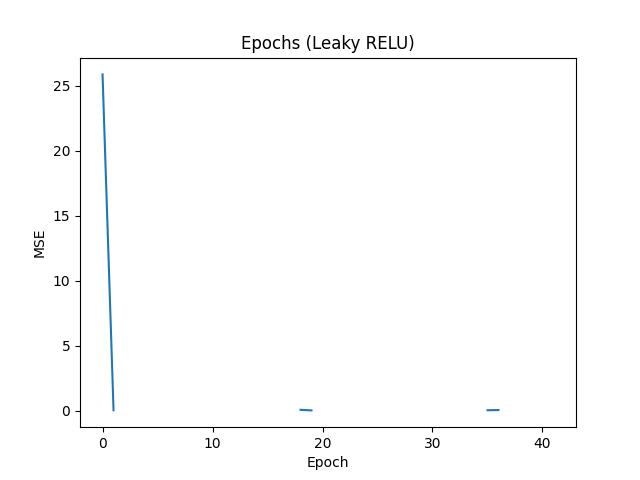
\includegraphics[width=0.45\textwidth]{FYS-STK/Prosjekt_2/Epochs (Leaky RELU).png}
\caption{Figure 14: Plot of change in MSE when varying amount of epochs for our neural network using the leaky relu function.}
\\
\\
On these plots, including the heatmap, we clearly see the leaky relu function converging a lot, and only a few of the epochs give a good result. This could be due to the fact that leaky relu never returns a $0$ value in the derivative unless our input value is $0$. This means if the network starts to converge, our network will not be able to stop it by saturating the neurons like sigmoid and relu can. 
\\
\\
However looking at the epochs plot for relu, we see a more stable estimation than with sigmoid. Even though our heatmap shows a bit worse results all over, in general, relu seems to be more stable and predictable. This shows us that maybe we were just lucky with our data set and sigmoid simulation, but for different regression problems where the data sets vary more, relu might prove to be a better option. 
\\
\\
We seem to have found the best contender for regression problems, being our neural network using either sigmoid or relu. We will therefore move on to classification problems, where we will compare with logistic regression. We start by simulating our breast cancer data set for our neural network, for every activation function.

%\begin{figure}[H]
%    \centering
%    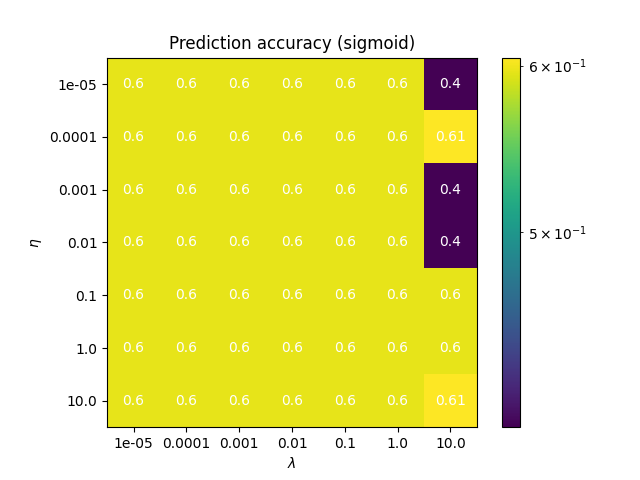
\includegraphics[width=0.45\textwidth]{FYS-STK/Prosjekt_2/Prediction accuracy (sigmoid).png}
%    \caption{Plot of change in accuracy when varying $\lambda$ (momentum) and learning rate for our neural network using sigmoid function.}
%    \label{fig:15}
%\end{figure}
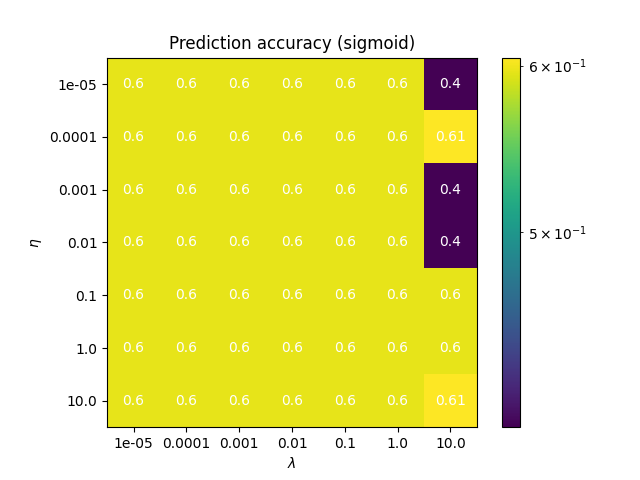
\includegraphics[width=0.45\textwidth]{FYS-STK/Prosjekt_2/Prediction accuracy (sigmoid).png}
\caption{Figure 15: Plot of change in accuracy when varying $\lambda$ (momentum) and learning rate for our neural network using sigmoid function.}

%\begin{figure}[H]
%    \centering
%    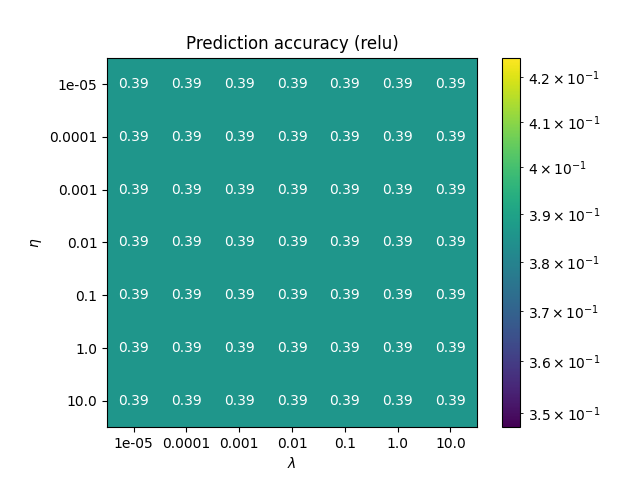
\includegraphics[width=0.45\textwidth]{FYS-STK/Prosjekt_2/Prediction accuracy (relu).png}
%    \caption{Plot of change in accuracy when varying $\lambda$ (momentum) and learning rate for our neural network using relu function.}
%    \label{fig:16}
%\end{figure}
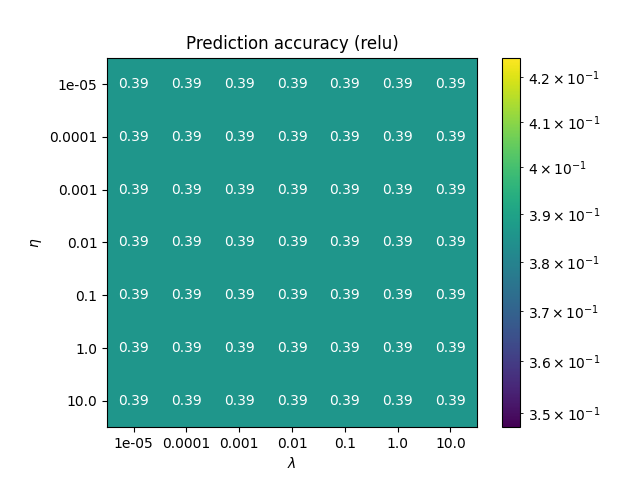
\includegraphics[width=0.45\textwidth]{FYS-STK/Prosjekt_2/Prediction accuracy (relu).png}
\caption{Figure 16: Plot of change in accuracy when varying $\lambda$ (momentum) and learning rate for our neural network using relu function.}

%\begin{figure}[H]
%    \centering
%    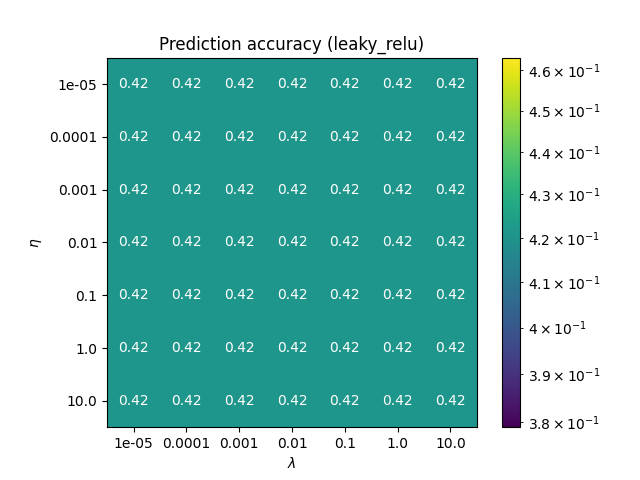
\includegraphics[width=0.45\textwidth]{FYS-STK/Prosjekt_2/Prediction accuracy (leaky_relu).png}
%    \caption{Plot of change in accuracy when varying $\lambda$ (momentum) and learning rate for our neural network using the leaky relu function.}
%    \label{fig:17}
%\end{figure}
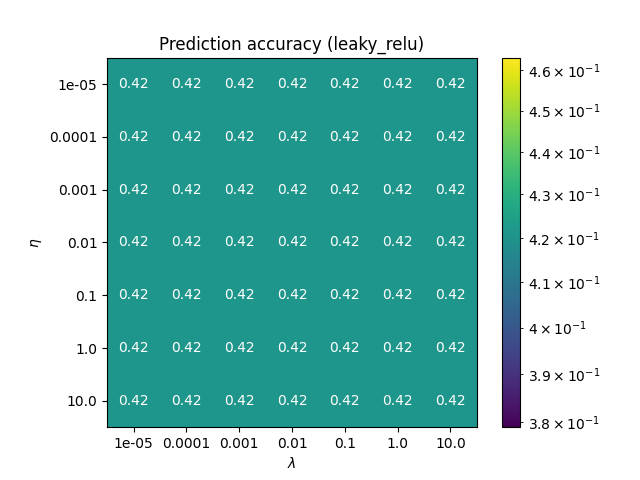
\includegraphics[width=0.45\textwidth]{FYS-STK/Prosjekt_2/Prediction accuracy (leaky_relu).png}
\caption{Figure 17: Plot of change in accuracy when varying $\lambda$ (momentum) and learning rate for our neural network using the leaky relu function.}
\\
\\
These results are not very impressive. It seems as though our neural network does not handle either classification or the data set very well. We see this if we also make the confusion matrix. We do a simulation using the sigmoid function and get an accuracy of $67 \%$, which in theory is ok, but the confusion matrix we get is
\begin{bmatrix}
    0 & 38\\
    0 & 76
\end{bmatrix}
which shows us that the classifier only assigned points to one class. The cause of this could also be that the data set is too uneven, or that we were not able to find suitable parameters for our neural network. We now compare these results with sklearn's own neural network model, using different layer sizes.

%\begin{figure}[H]
%    \centering
%    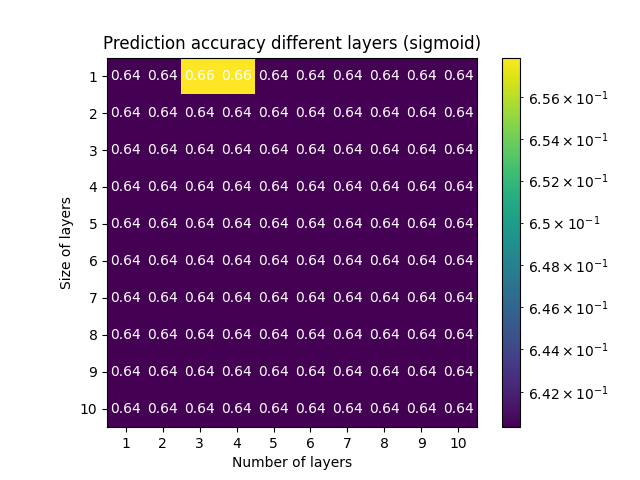
\includegraphics[width=0.45\textwidth]{FYS-STK/Prosjekt_2/Prediction accuracy different layers (sigmoid).png}
%    \caption{Plot of change in accuracy when varying the layer sizes and number of layers for our neural network using the sigmoid function.}
%    \label{fig:18}
%\end{figure}
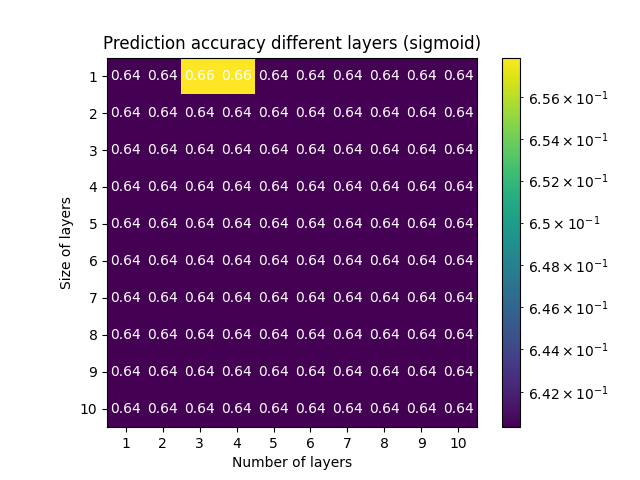
\includegraphics[width=0.45\textwidth]{FYS-STK/Prosjekt_2/Prediction accuracy different layers (sigmoid).png}
\caption{Figure 18: Plot of change in accuracy when varying the layer sizes and number of layers for our neural network using the sigmoid function.}

%\begin{figure}[H]
%    \centering
%    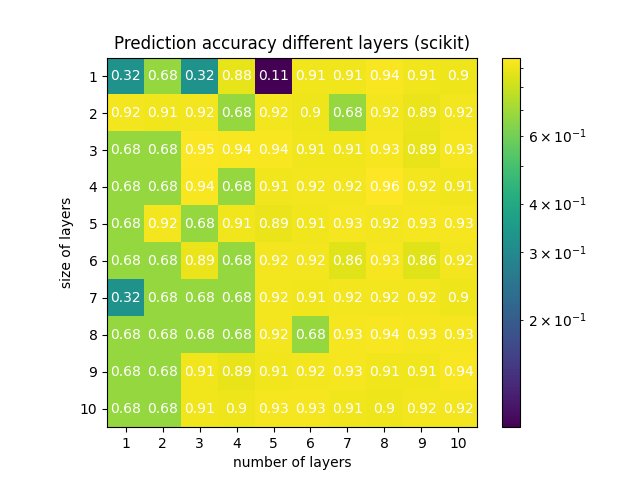
\includegraphics[width=0.45\textwidth]{FYS-STK/Prosjekt_2/Prediction accuracy different layers (scikit).png}
%    \caption{Plot of change in accuracy when varying the layer sizes and number of layers for scikits model using sigmoid function.}
%    \label{fig:19}
%\end{figure}
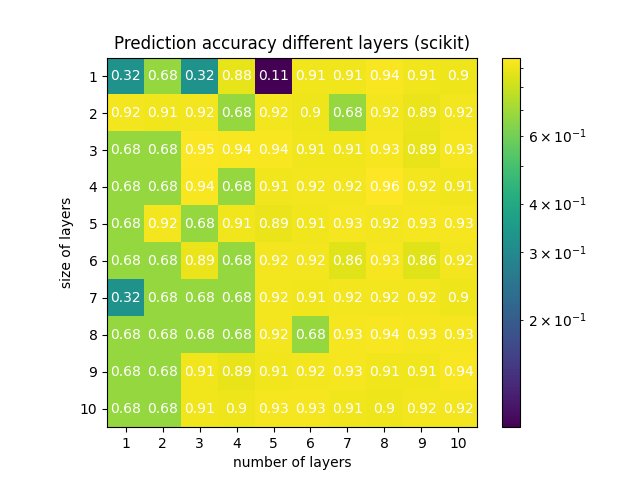
\includegraphics[width=0.45\textwidth]{FYS-STK/Prosjekt_2/Prediction accuracy different layers (scikit).png}
\caption{Figure 19: Plot of change in accuracy when varying the layer sizes and number of layers for scikits model using sigmoid function.}
\\
\\
Here we see the same pattern we were hoping not to get. It seems as though our neural network really does classify by assigning only one class. However, when studying the predictions done by scikit, we see a similar patter in accuracy. Even though the scikit model is able to give a very good prediction with $90 \%$ accuracy most of the time, we see that a lot of the layer choices gives the same accuracy that we got with our own network, or worse. This could indicate to us that our neural network predicts only one class because its an easy prediction due to the data set being uneven, and that if we did quite a bit more simulations we might end up with parameters that could give decent results.
\\
\\
However, the last model we implemented was logistic regression. Here we have results from our own logistic regression and scikits logistic regression model.

%\begin{figure}[H]
%    \centering
%    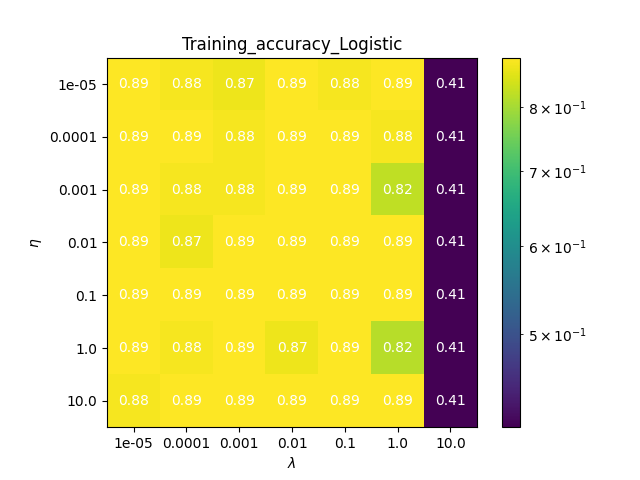
\includegraphics[width=0.45\textwidth]{FYS-STK/Prosjekt_2/Training_accuracy_Logistic.png}
%    \caption{Plot of change in accuracy for our logistic regression method when varying the learning rate ($\eta$) and the l2 regularization parameter $\lambda$.}
%    \label{fig:20}
%\end{figure}
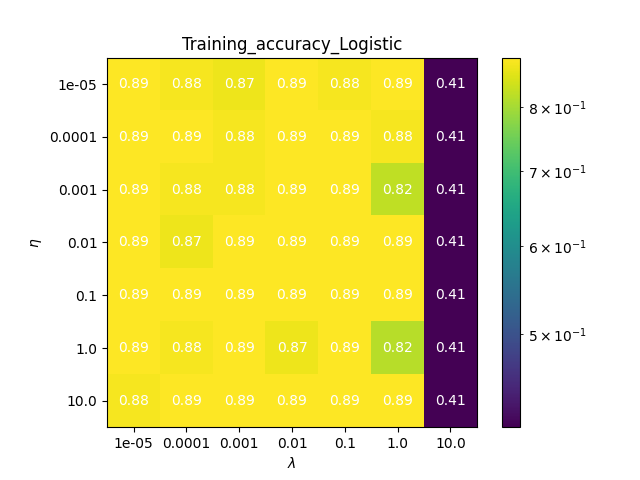
\includegraphics[width=0.45\textwidth]{FYS-STK/Prosjekt_2/Training_accuracy_Logistic.png}
\caption{Figure 20: Plot of change in accuracy for our logistic regression method when varying the learning rate ($\eta$) and the l2 regularization parameter $\lambda$.}

%\begin{figure}[H]
%    \centering
%    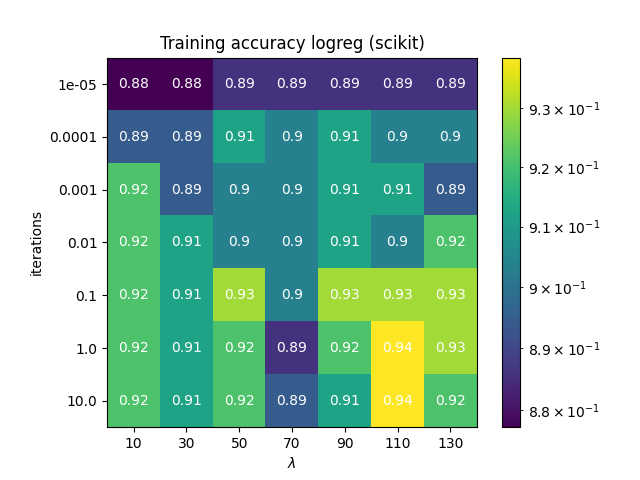
\includegraphics[width=0.45\textwidth]{FYS-STK/Prosjekt_2/Training accuracy logreg (scikit).png}
%    \caption{Plot of change in accuracy for scikits logistic regression method when varying the number of iterations and the l2 regularization parameter $\lambda$.}
%    \label{fig:21}
%\end{figure}
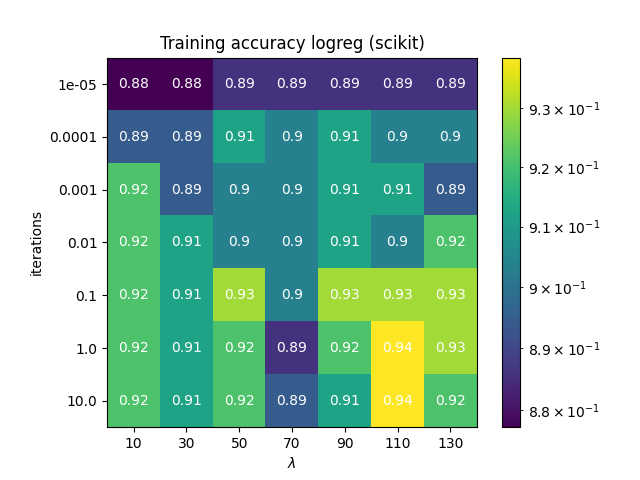
\includegraphics[width=0.45\textwidth]{FYS-STK/Prosjekt_2/Training accuracy logreg (scikit).png}
\caption{Figure 21: Plot of change in accuracy for scikits logistic regression method when varying the number of iterations and the l2 regularization parameter $\lambda$.}
\\
\\
As we see from these results, our logistic regression method is able to produce results about as good as scikits own neural network and scikits logistic regression. We also see here for $\lambda = 10$ that we get a pattern of predicting only one class, further adding to our suspicion that the data set is not balanced, but this could also just be because a $\lambda$ of 10 is so high that the model easily converges towards one single solution. We see however that our logistic regression is very stable at producing good results. This shows us that logistic regression is a very good method for classification, and seems to be the best one out of the models we implemented, at least for these data sets.

\section{CONCLUSION}\label{sec:CONCLUSION}
During this project we saw the importance of tuning the learning rate, choosing correct parameters, and also looking at different activation functions. Our results seem to indicate that our neural network implementation was the best at handling regression, but was difficult to use for classification problems, at least with huge and complex data sets, where instead our logistic regression worked best. There could have been some faulty implementation or poor choice of parameters that made our neural network not function as well on classification, seeing as scikits neural network worked fine. If we managed to fix our network more it could have also shown us bigger differences in the activation function, since we were not able to study them that much. However, this project showed us how well a neural network can work when implemented correctly, and proved to us that they are worth the implementation hassle. 

\section{CODE}\label{sec:CODE}
The code used to simulate can be found at \href{https://github.com/erlend1202/FYS_STK4155_Prosjekt_2}{this} Github repository.

\section{REFERENCES}\label{sec:REF}
Goodfellow et al \href{https://www.deeplearningbook.org/}{Deep Learning}, (MIT Press, 2016).\label{ref:Goodfellow et al}
\\
Hjorth-Jensen, Morten \href{https://compphysics.github.io/MachineLearning/doc/LectureNotes/_build/html/intro.html}{Applied Data Analysis and Machine Learning}, (2021) \label{ref:Morten}
\\
T.Hastie \href{https://hastie.su.domains/Papers/ESLII.pdf}{The Elements of Statistical Learning}, second edition, (Springer, 2001).\label{ref:HASTIE}
\\
S.Dorsaf \href{https://medium.com/analytics-vidhya/comprehensive-synthesis-of-the-main-activation-functions-pros-and-cons-dab105fe4b3b}{Comprehensive synthesis of the main activation functions pros and cons}, (Apr 2, 2020).\label{ref:DORSAF}




\appendix

\section{Numerical Notation}\label{sec:NOTATION}
\caption{Franke function:}
\label{eq:FrankeFunction}
\begin{align*}
    f(x,y) &= \frac{3}{4} exp \left( \frac{(9x -2)^2}{4} - \frac{(9y -2)^2}{4}  \right) \\
    &+  \frac{3}{4} exp \left( -\frac{(9x + 1)^2}{49} - \frac{(9y + 1)}{10} \right) \\
    &+ \frac{1}{2} exp \left( -\frac{(9x -7)^2}{4} - \frac{(9y - 3)^2}{4} \right) \\
    &- \frac{1}{5} exp \left( - (9x - 4)^2 - (9y - 7)^2 \right)
\end{align*}

\end{document}